\chapter{人与自然}\label{ch:g5:people-and-nature}

站在山顶俯瞰山谷：田地整齐如方格，
林地经过管理，河岸被拉直，道路纵横，
屋顶错落。放眼望去，几乎没有一处是自然生长成这样的。人类
是唯一一种按自身需要重塑整片景观的\omterm{def:g5:biodiversity:species}{物种}。
本章要客观审视这种力量：
它带给我们什么，付出什么代价，又该如何善加利用。

\section{人类塑造的景观}

\begin{proposition}[大多数景观都经过人为管理]\label{prop:g5:people-and-nature:managed}
我们身边几乎所有景观都受到人类塑造：
\begin{itemize}
  \item \emph{田地}\index{田地}是经过管理的土地，
        人们选种一种作物——小麦、玉米、马铃薯——
        来代替野生的混合植被；
  \item 大多数\emph{森林}\index{森林（经管理的）}是
        人工种植、间伐并采伐的，如同生长缓慢的作物；
  \item \emph{草地}之所以存在，是因为它们会被割草或放牧，
        ——一旦被弃置，就会先长成灌丛，
        再发展为林地；
  \item 城镇、道路和水坝重新规划了土地本身。
\end{itemize}
“未被触动”的角落只是例外，大多数
还是人为刻意保护的。
\end{proposition}
\admitted

\begin{example}[读懂山谷]\label{ex:g5:people-and-nature:valley}
山顶这幅景象，逐项来看：小麦田供应
面包店；云杉成行，是比护林员年纪还大的木材作物；
开花的草地每年七月割一次，连续两个夏天不割，
荆棘便会蔓延过来；河流很久以前就被拉直，
以保护田地免受洪水侵袭。山谷就是一座
车间，而且已经运转了几个世纪。
\end{example}

\begin{omfigure}
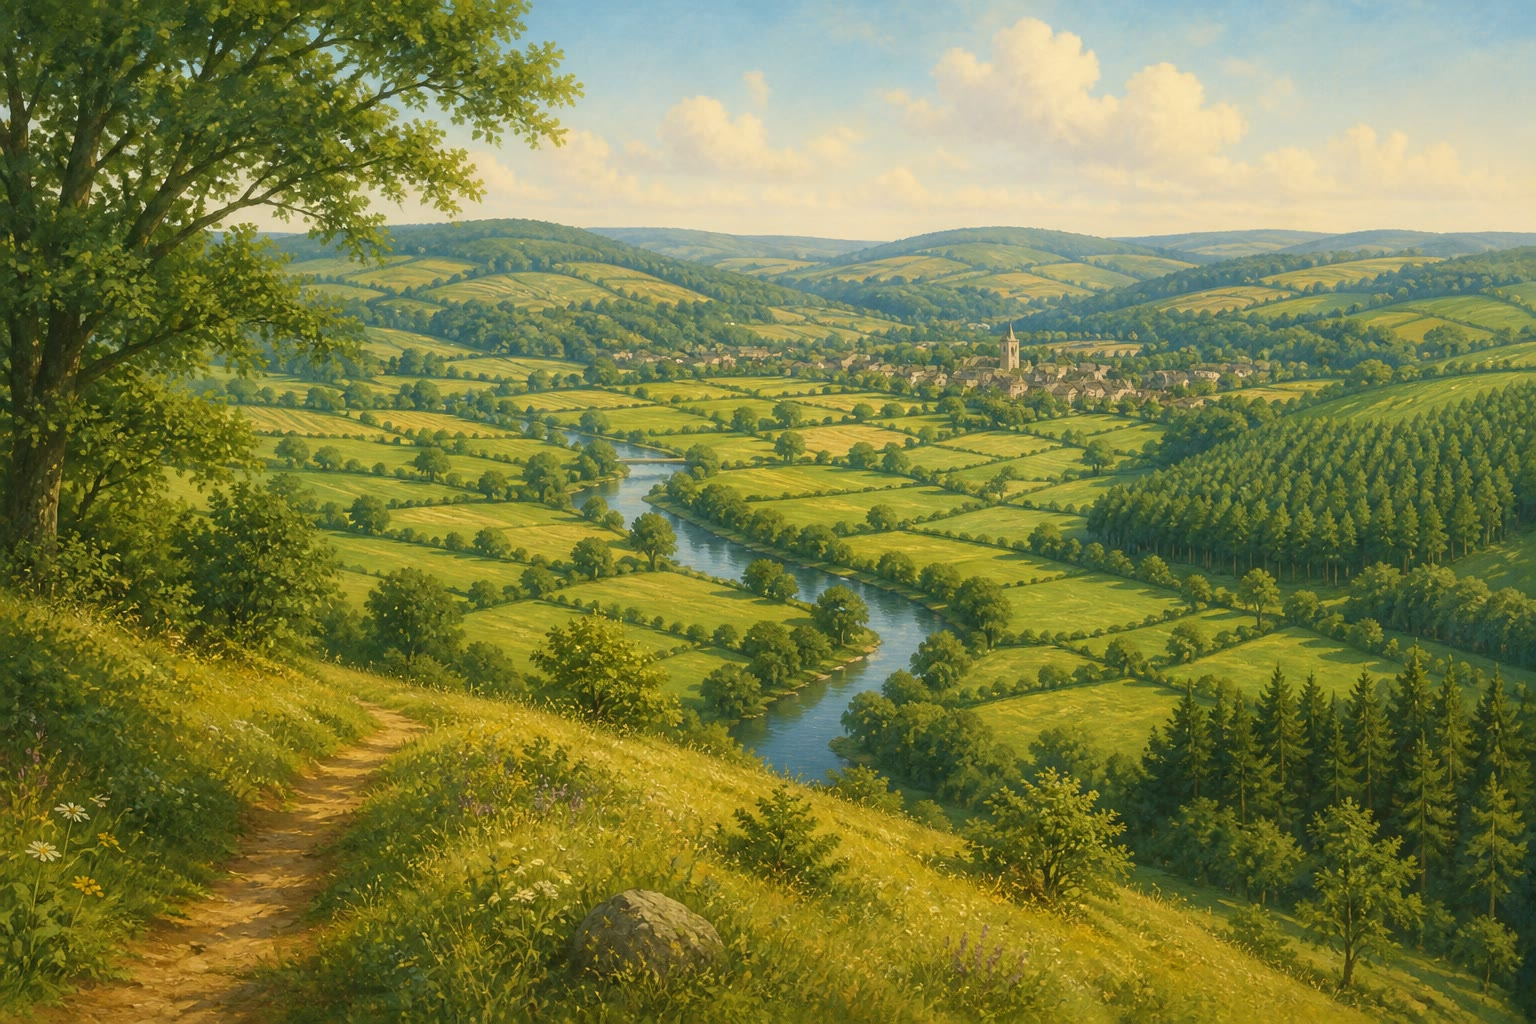
\includegraphics[width=0.62\linewidth]{images/book1/ai/g5-nature-valley.jpg}

{\small 山顶俯瞰的景象：田地、树篱、经管理的
森林、拉直的河流、村庄——一片仍在运作的景观，
已有几个世纪之久。}
\end{omfigure}

\begin{remark}[既非反派，也非园丁]\label{rem:g5:people-and-nature:honest}
若把这段历史讲成纯粹的破坏，那是不实的——
农业养活了人类，而有树篱的农田
可以拥有丰富的\omterm{def:g5:biodiversity:species}{物种}（见\cref{ex:g5:biodiversity:orchard}）——同样，
假装改造不需要付出代价，也是不实的
（\cref{prop:g5:biodiversity:loss}中已列出这些代价）。这里的
真正诚实的问题从来不是“要不要触动自然？”，而是“如何
管理我们所触动的东西，使其持续发挥作用——既为我们，
也为\omterm{def:g5:food-webs:web}{食物网}中的其他\omterm{def:g1:living-or-not:living}{生物}？”
\end{remark}

\section{善加管理与管理不善}

\begin{example}[山坡耕作的两种方式]\label{ex:g5:people-and-nature:twofarms}
山坡甲：一整块大田，树篱被铲除，土壤整个冬天裸露。
雨水把松动的土壤冲向坡下；
\cref{ex:g5:biodiversity:orchard}中的帮手们失去了栖身之所；
一种害虫便可毫无阻碍地席卷这一单一作物。山坡乙：
田块较小，保留树篱，冬季土壤有覆盖，
作物逐年轮作。树篱固定土壤，并为
捕食害虫的\omterm{def:g1:animals-around-us:animal}{动物}提供住所；轮作让土地得以休养。两块
山坡都能养活人——只有一块在一百年后仍能如此。
\end{example}

\begin{proposition}[持久利用的三条规则]\label{prop:g5:people-and-nature:lasting}
自然资源能够持久利用，前提是遵守三条规则：
\begin{enumerate}
  \item \emph{索取速度不超过其更新速度}：按森林的生长速度采伐木材，
        按鱼群的繁殖速度捕鱼——
        捕捞过度（见\cref{prop:g5:biodiversity:loss}）
        就是违反了这条规则；
  \item \emph{保护帮手}：土壤\omterm{def:g1:living-or-not:living}{生物}、\omterm{def:g5:flower-to-fruit:steps}{传粉}者、食虫\omterm{def:g1:animals-around-us:animal}{动物}
        ——这些免费服务见
        \cref{exo:g5:biodiversity:11}——这些服务需要它们的栖身之所
        得以保留；
  \item \emph{归还所借之物}：堆肥的物质循环，
        在各个尺度上都要如此（见\cref{rem:g4:what-plants-need:soil}）。
\end{enumerate}
\end{proposition}
\admitted

\begin{example}[护林员的算账]\label{ex:g5:people-and-nature:forester}
管理良好的森林，是第一条规则行之有效的最古老证明：
护林员每年清点森林的生长量，砍伐量
绝不超过这一数量。这样，森林每年都能
提供木材，并且永远如此——它始终是森林，
有猫头鹰、鹿和甲虫。世界上有一些经管理的森林，
已这样采伐了数百年，
而森林并未因此缩小。
\end{example}

\section{城市，以及重新腾出空间}

\begin{example}[城镇中的自然]\label{ex:g5:people-and-nature:city}
城市看上去与自然截然相反，但它也是一种\omterm{def:g2:where-animals-live:habitat}{栖息地}，
——一种奇特的岩石质\omterm{def:g2:where-animals-live:habitat}{栖息地}。雨燕把巢筑在混凝土“峭壁”上，
狐狸在垃圾桶之间巡行，野生\omterm{def:g1:plants-around-us:plant}{植物}从沥青接缝处钻出。
居民也可以扩大对野生\omterm{def:g1:living-or-not:living}{生物}的接纳：
公园、绿色屋顶、为蜜蜂种的阳台花卉，还有
\cref{ex:g2:where-animals-live:schoolpond}中的校园池塘。
\cref{met:g5:biodiversity:help}中的方法，
同样适用于建筑之间。
\end{example}

\begin{example}[让河流重获河湾]\label{ex:g5:people-and-nature:river}
山谷里那条被裁直的河流水流湍急，下游洪涝严重，
河湾消失后，\omterm{prop:g3:sorting-living-things:groups}{鱼类}和蜻蜓也随之消失。
工程师现在有时会\emph{重新弯曲}这类河流：
恢复的弯道和湿草甸能减缓水流、蓄存洪水，
\cref{ex:g5:biodiversity:storks}中的鹳
又能找到它们的草甸。管理也可以反过来进行——
修复本身也是一种管理。
\end{example}

\begin{method}[判断对自然的利用]\label{met:g5:people-and-nature:judge}
对于任何土地或水体的利用——农场、渔场、
规划中的道路、花园等，应依次追问：
\begin{enumerate}
  \item 问：什么被\emph{取用}，取用是否快于其
        再生速度（规则 1）；
  \item 问什么\emph{\omterm{def:g2:where-animals-live:habitat}{栖息地}与劳动者}得以保留或丧失
        （规则 2）；
  \item 问什么被\emph{归还}——又留下了哪些废弃物
        （规则 3）；
  \item 最后判断：这种做法能否持续一百年？
        哪一项改变最能改善这一结论？
\end{enumerate}
\end{method}

\section{练习}

\begin{exercise}[$\star$]\label{exo:g5:people-and-nature:1}
请从
\cref{prop:g5:people-and-nature:managed}中列出四种人为塑造的景观，
并说明每种景观的管理目的。
\end{exercise}

\begin{exercise}[$\star$]\label{exo:g5:people-and-nature:2}
若草甸不再被刈割或放牧，会发生什么？
\end{exercise}

\begin{exercise}[$\star$]\label{exo:g5:people-and-nature:3}
说明可持续利用的三条规则。
\end{exercise}

\begin{exercise}[$\star$]\label{exo:g5:people-and-nature:4}
在\cref{ex:g5:people-and-nature:twofarms}中，
列出两处山坡之间的三项差异，
以及每项差异会引起什么改变。
\end{exercise}

\begin{exercise}[$\star$]\label{exo:g5:people-and-nature:5}
解释林务员的算账方法。它属于哪条规则，
作为回报，森林能提供多少产量——能持续多久？
\end{exercise}

\begin{exercise}[$\star$]\label{exo:g5:people-and-nature:6}
列出三种城市中的野生\omterm{def:g1:living-or-not:living}{生物}，并说明各自
利用城市的哪一特征作为\omterm{def:g2:where-animals-live:habitat}{栖息地}。
\end{exercise}

\begin{exercise}[$\star$]\label{exo:g5:people-and-nature:7}
重新弯曲河流恢复了什么——对人类和
对\omterm{def:g5:food-webs:web}{食物网}分别有何作用？
\end{exercise}

\begin{exercise}[$\star$]\label{exo:g5:people-and-nature:8}
试一试：选取家附近的一处景色——街道、田野、公园——
列出其中所有受人类管理的事物，如
\cref{ex:g5:people-and-nature:valley}所示；
有没有未被管理的事物？
\end{exercise}

\begin{exercise}[$\star\star$]\label{exo:g5:people-and-nature:9}
“保护自然意味着永远不去触碰它。”请结合
\cref{prop:g5:people-and-nature:managed}中被刈割的草甸讨论，
这类\omterm{def:g2:where-animals-live:habitat}{栖息地}
若无人为干预便会\emph{消失}，并
结合\cref{rem:g5:people-and-nature:honest}。
\end{exercise}

\begin{exercise}[$\star\star$]\label{exo:g5:people-and-nature:10}
运用\cref{met:g5:people-and-nature:judge}，
对\cref{ex:g5:people-and-nature:twofarms}中的山坡 A 进行判断：
它违反了哪些规则，以及哪一项改变最能改善它？
\end{exercise}

\begin{exercise}[$\star\star\star$]\label{exo:g5:people-and-nature:11}
某渔船队的渔获量连续五年翻倍，形势极好；
第六年，鱼群消失，船队闲置。
试用规则 1 解释这六年的变化——为何违反该规则
起初反而\emph{看似}成功？并与林务员
相反的算账方法作比较。
\end{exercise}
